\documentclass{article}
\usepackage{cancel}
\usepackage{gensymb}
\usepackage{tikz}
\usetikzlibrary{angles,quotes}
\usetikzlibrary{arrows.meta,calc}


\renewcommand{\thesubsubsection}{\alph{subsubsection})}

\title{Astro HW 7}
\author{Pierson Lipschultz}

\begin{document}
\maketitle
\setcounter{section}{7}

\subsection{}


\subsubsection{}

%  check this, random diff component needed for the star being greater mass, unsure where that eq comes from
\begin{center} 
    \(P = 4.727\) days \(\times \frac{1 year}{365.25days} = .001294\) years \\
    \(\frac{a^3}{1.09 M_\odot} = p^2, a = (.001294^2 \times 1.09 ^{1/3}\) \\
    \(.056\)AU 
\end{center}

\subsubsection{}

\begin{center}
    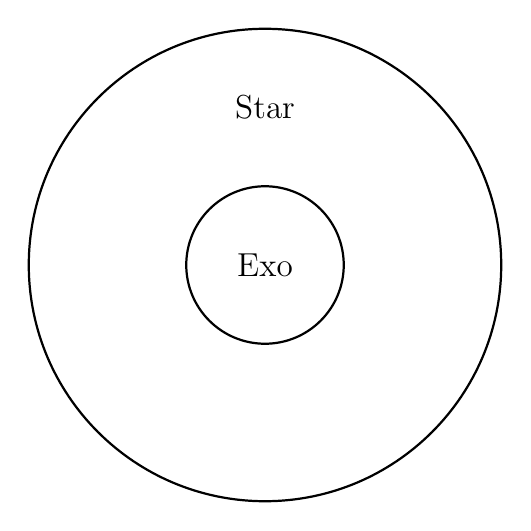
\begin{tikzpicture}[line cap=round,line join=round]
    
    % circles
    \draw[thick] (0,0) circle (3cm); % outer (Star)
    \draw[thick] (0,0) circle (1cm); % inner (Exo)
    
    % labels
    \node[font=\large] at (0,2) {Star};
    \node[font=\large] at (0,0) {Exo};
    
    \end{tikzpicture}\\
    Probably didn't need to derive this, but it was a fun derivation, so oh well. \\
    Find 2d projection areas of the star and the planet, then calculate what percentage of the area of the star is covered, then use that to get planet radius.\\
    \(A_s = 2\pi r_s^2\)\\
    \(A_p = 2\pi r_p^2\)\\
    \(A_s \times \delta = A_p\)\\
    \(r_p = r_s \sqrt{\delta}\) \\
    \(r_s = .98 \times 6.944 \times 10^5km\)\\
    \(r_p = 680512km\sqrt{2.2\times10^{-4}}\)\\
    \(r_p = 10093.62km\)
\end{center}

\subsubsection{}

\begin{center}

\end{center}

\subsubsection{}

\begin{center}
    
\end{center}

\subsection{}
\subsubsection{}
\begin{center}
    \(L = 4\pi R^2\sigma_{sb} T^4\)\\
    \(\frac{1}{R^2} = \frac{4\pi\sigma_{sb} T^4}{L}\) \\
    \({R^2} = \frac{L}{4\pi\sigma_{sb} T^4}\)\\
    \({R} = \sqrt{\frac{L}{4\pi\sigma_{sb} T^4}}\)
    \vspace{5mm} \\
    \(R_a = \sqrt{\frac{1.1 \times 10^{26}}{4\pi \sigma_{sb} 3200^4}}\)\\
    \(R_a = 1.213 \times 10^{9}\)m\\
    \vspace{5mm}
    \(R_b = \sqrt{\frac{5.2 \times 10^{25}}{4\pi \sigma_{sb} 32^4}}\)\\
    \(R_b = 8.34 \times 10^{12}\)m
    \end{center}

\subsubsection{}
\begin{center}
    One of the radii is very similar to the sun,  The Sun has a radius of \(\approx 6.95 \times 10 ^8\), so it's about double. 

    However, \(R_b\) is \textbf{much} larger than our sun, by four orders of magnitude.

\end{center}

\subsection{}
\subsubsection{}

\begin{center}


    \begin{tikzpicture}[scale=3, thick]
    
    % --- Adjustable parameters ---
    \def\base{3}  % base length (arbitrary scale)
    \def\height{1}  % height (AU)
    
    \def\baseName{\(7.7 \times 10^{16}m\)}
    \def\heightName{\(a\)}
    \def\thetaName{\(6''\)}

    % --- Coordinates ---
    \coordinate (A) at (0,0);          % left vertex
    \coordinate (B) at (\base,0);      % right vertex on x-axis
    \coordinate (C) at (\base,\height);% top vertex
    
    % --- Triangle ---
    \draw[thick] (A)--(B)--(C)--cycle;
    
    % --- Right-angle marker ---
    \draw ($(B)!0.15!(A)$) -- ++(0,0.15) -- ($(B)!0.15!(C)$);
    
    % --- Angle label (6.0'') ---
    \draw[->,thin] (0.5,0) arc[start angle=0,end angle=atan(\height/\base),radius=0.5];
    \node at (0.3,0.18) [font=\footnotesize] {\thetaName};
    
    % --- Axis labels ---
    \draw[->] (-0.2,0) -- (\base+0.5,0) node[right] {$x$};
    \draw[->] (0,-0.2) -- (0,\height+0.5) node[above] {$y$};
    
    % --- Side labels ---
    \node[below] at ($(A)!0.5!(B)$) {\baseName};
    \node[right] at ($(B)!0.5!(C)$) {\heightName};
    
    \end{tikzpicture}
    \(d = \frac{1}{.4}\)parsecs\\
    \(d = 2.5\)parsecs\\
    \(d = 2.5 * 3.086* 10 ^{16}\)m\\
    \vspace{6mm}

    \(a = 2.39 \times 10^{12}\)m \\

    \vspace{6mm}
    
    \(P^2 = \frac{4\pi ^2 a^3}{GM}\)\\
    \(M = \frac{4\pi^2 a^3}{Gp^2}\)\\
    \(P = 80 \times 365.25 \times 24 \times 3600\)yr \\
    \vspace{6mm}
    \(M_{tot} = 1.234 \times 10^{30}\)kg
\end{center}

\subsubsection{}
    \begin{center}
        Because we are assuming the orbits are circular and are effectively calculating the stars muddled together. If we had, for example, vectors of each, and thus eccentricity, we could find the gravitational pulls of each of the stars, and thus find the masses.
    \end{center}
\subsection{}
\subsubsection{}


\end{document}
